\subsection{Experiment 7C: complementary local operating coverage}
\label{sec:experiment7c}

\paragraph{Question and frozen gate.}
Experiments 7A and 7B show that six seconds over three nearby speeds already
suffice for accurate local structured identification. Experiment 7C therefore
tests the more restrictive premise needed by the federated argument: can
compatible clients compensate for operating regions that a recipient never
observes? The primary gate requires oracle Family pooling to reduce mean
held-out tracking error relative to Local by at least 5\%, with a positive
lower 95\% paired-seed bootstrap bound, amplitude feasibility, and maximum
frozen spectral radius below one. The gate and protocol were fixed before the
ten new fleets (seeds 51--60) were evaluated.

\paragraph{Complementary data and controls.}
Each of the ten clients in an oracle family is assigned one constant collection
speed from $\{10,12,14,16,18,22,24,26,28,30\}$ m/s and records three independent
one-second steering episodes only at that speed. Thus a Local fit receives 300
transitions from a single speed, whereas a Family fit receives 3,000 transitions
whose union covers the full envelope. Global pools all three families. As an
information-budget control, LocalExtra gives every recipient 3,000 transitions
collected from that same vehicle over all ten speeds. It is an oracle for the
value of additional local calibration, not a deployable federated method.
All fits use the unchanged bounded three-ratio output-error estimator, noise
levels, controller synthesis, three 24-second held-out scenarios, amplitude
checks, and 161-speed frozen stability audit. Test trajectories are generated
only after identification. No test metric enters model fitting or selection.

\paragraph{Results.}
All 640 fits converge from both starts without bound hits; the largest relative
multistart difference is $2.46\times10^{-7}$. All 3,600 closed-loop evaluations
are amplitude-feasible and the maximum frozen spectral radius is 0.96938.

\begin{table}[htbp]
\centering
\caption{Experiment 7C on ten new fleets. Tracking reports mean $\pm$ sample
standard deviation across fleet seeds. Parameter error is componentwise relative
error. LocalExtra has the same transition count as Family but uses recipient-local
full-envelope data.}
\label{tab:experiment7c}
\begin{tabular}{lrrr}
\toprule
Method & Tracking [deg/s] & Yaw prediction [deg/s] & Parameter error\\
\midrule
Local & $0.006703\pm0.000052$ & 0.04931 & 1.499\%\\
Global & $0.011755\pm0.000465$ & 0.36889 & 7.383\%\\
Family & $0.007615\pm0.000127$ & 0.15873 & 2.617\%\\
LocalExtra & $0.006683\pm0.000051$ & 0.04792 & 0.478\%\\
\bottomrule
\end{tabular}
\end{table}

\begin{figure}[htbp]
\centering
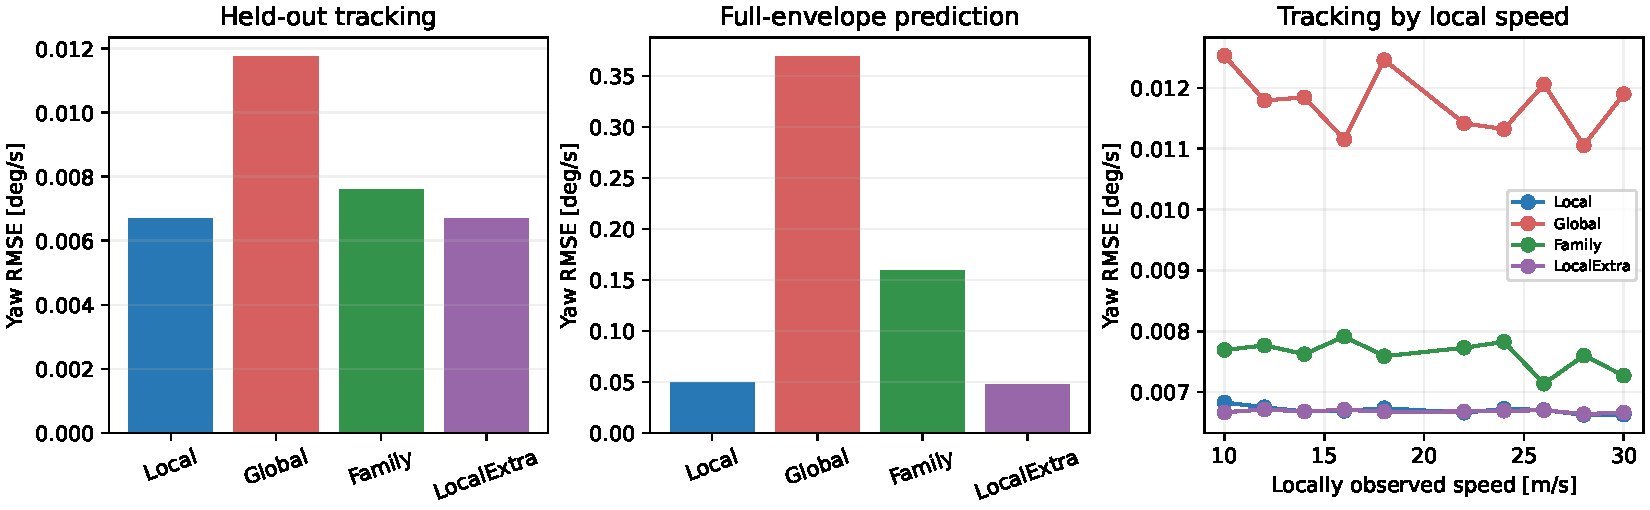
\includegraphics[width=\linewidth]{../results/figures/experiment_7c_complementary_coverage.pdf}
\caption{Experiment 7C held-out tracking, full-envelope common-input prediction,
and tracking grouped by the client's single observed speed. Tracking error bars
in the first panel show standard deviation across ten fleets.}
\label{fig:experiment7c}
\end{figure}

\Cref{tab:experiment7c,fig:experiment7c} shows that Family pooling improves
tracking by 35.22\% relative to Global, with all ten paired fleets favorable.
It nevertheless increases tracking error by 13.61\% relative to Local. The
paired difference $J_{\rm Local}-J_{\rm Family}$ is
$-9.12\times10^{-4}$ deg/s, with 95\% bootstrap interval
$[-9.76\times10^{-4},-8.49\times10^{-4}]$ deg/s; none of the ten pairs favors
Family. The primary collaboration gate therefore fails. Family also has
221.91\% higher yaw-prediction error and 74.56\% higher relative parameter
error than Local. LocalExtra slightly improves tracking over Local and reduces
parameter error to 0.478\%, confirming that additional informative local data
remain useful even though their effect on closed-loop tracking is small.

\paragraph{Interpretation and decision.}
Complementary speed coverage is not the missing condition in this benchmark.
The known three-ratio bicycle structure lets a single-speed, three-second local
record identify a controller-relevant model accurately enough to extrapolate
over the full envelope. Pooling supplies speeds but also averages persistent
within-family parameter differences; here that bias is larger than the variance
removed by collaboration. The result is especially informative because it is
not caused by instability, infeasibility, an unlucky seed, or unequal data in
the Family--LocalExtra comparison.

Together, 7A--7C reject the current federated-accuracy route based only on finite
data, nearby-speed restriction, personalization, or complementary speed coverage.
An actual federated optimizer would approximate a centralized Family solution
whose accuracy gate has now failed repeatedly, so implementing it cannot repair
the statistical premise. The project should retain the oracle scheduling--
heterogeneity contribution and the negative sharing boundary. A further FL
study is justified only by a qualitatively different and application-grounded
information constraint, such as missing state labels, excitation directions
that make the local ratios unidentifiable, or a communication/deployment goal
that does not claim improved accuracy.

\paragraph{Reproducibility.}
The frozen protocol is \path{code/config/experiment_7c.json}. The runner is:
\begin{quote}\small
\path{code/experiments/experiment_7c_complementary_coverage.py}
\end{quote}
Set \texttt{PYTHONPATH} to \path{code/src:code/experiments}. The
\texttt{--summarize-only}
option rebuilds all aggregate tables and the figure. Compressed per-seed files
retain client metrics, fit diagnostics, prediction errors, local-speed assignments,
and transition-budget accounting. The conclusions file records hashes of the
protocol, runner, and estimator.
